\section{List$<$ Etype $>$ Class Template Reference}
\label{classList}\index{List@{List}}
{\tt \#include $<$link\-List.h$>$}

Inheritance diagram for List$<$ Etype $>$:\begin{figure}[H]
\begin{center}
\leavevmode
\includegraphics[width=117pt]{classList__inherit__graph}
\end{center}
\end{figure}
Collaboration diagram for List$<$ Etype $>$:\begin{figure}[H]
\begin{center}
\leavevmode
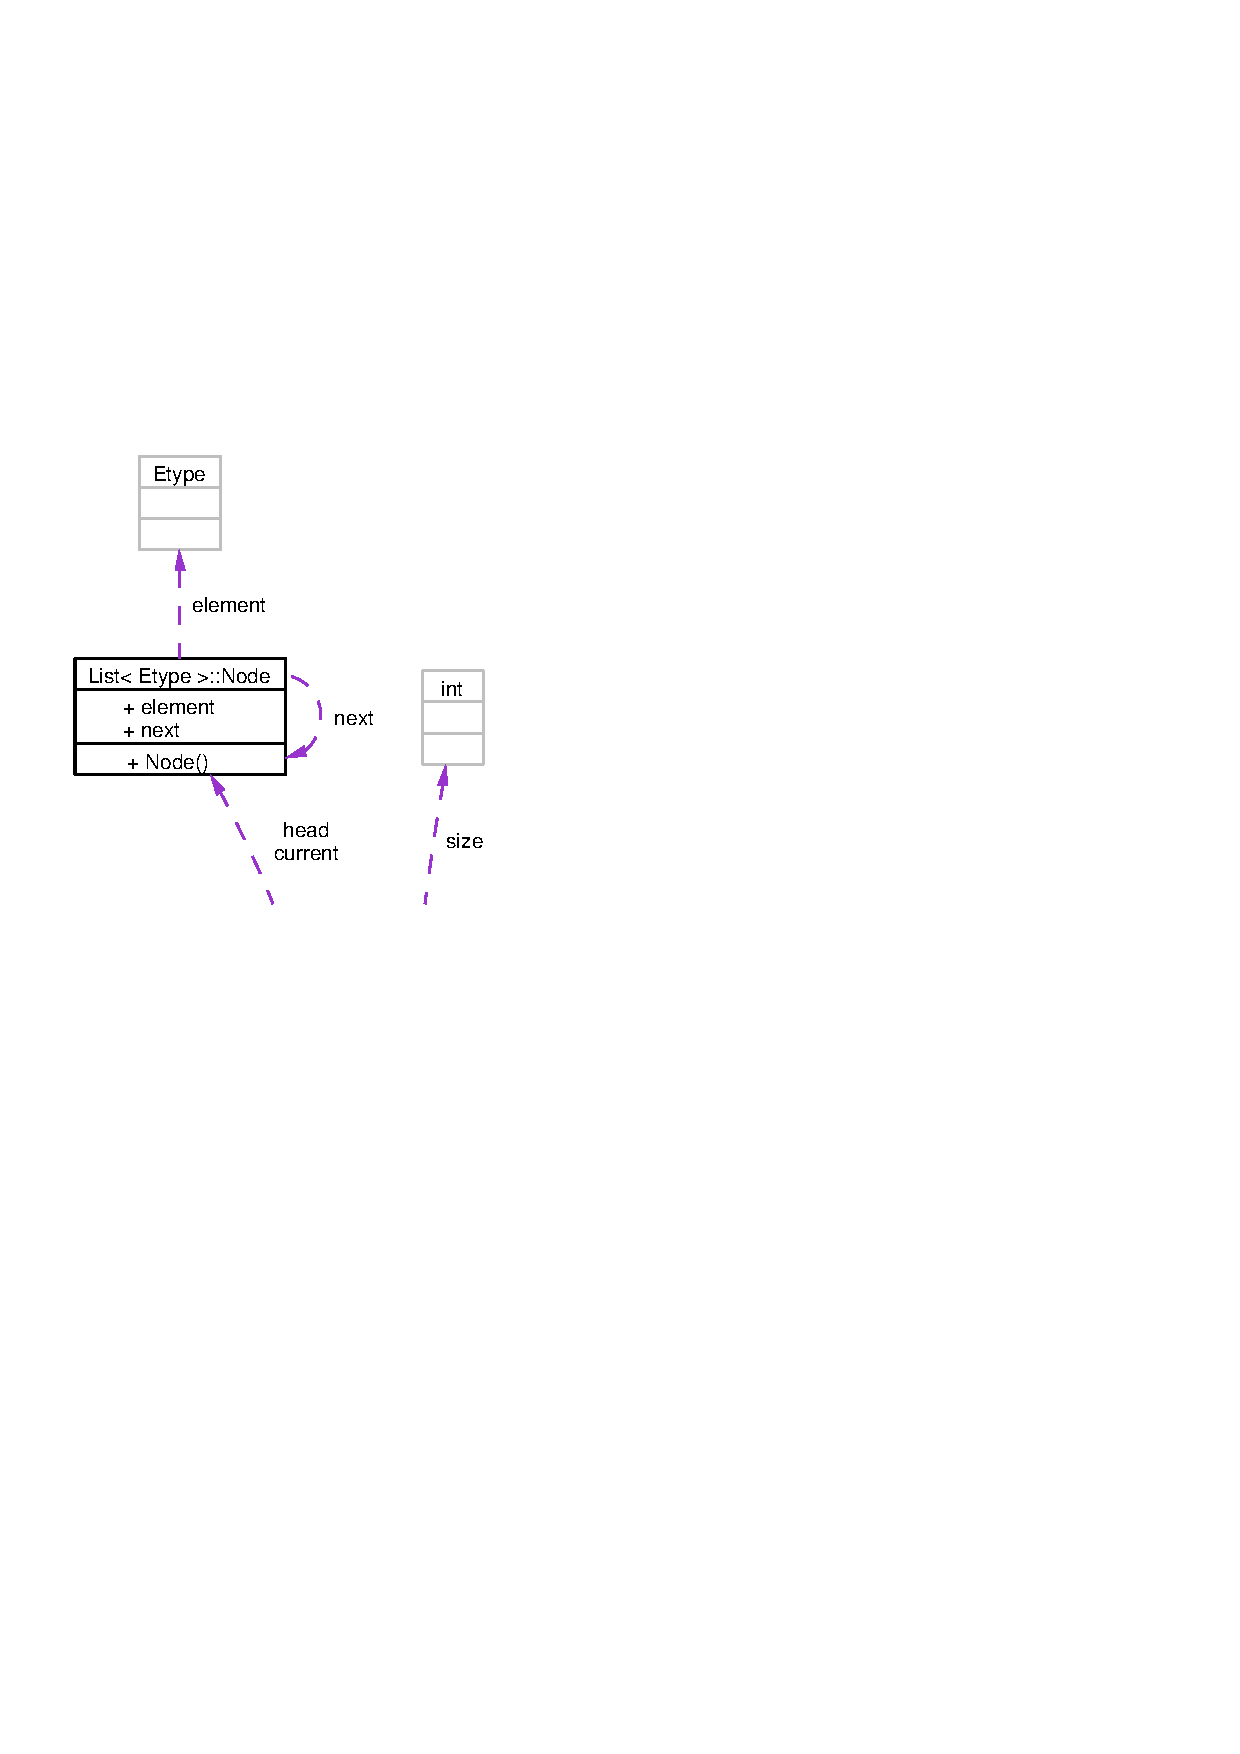
\includegraphics[width=122pt]{classList__coll__graph}
\end{center}
\end{figure}
\subsection*{Public Member Functions}
\begin{CompactItemize}
\item 
{\bf List} ()
\item 
{\bf List} (Etype a\-Low, Etype a\-High)
\item 
{\bf List} (const  {\bf List}$<$ Etype $>$ \&orig\-List)
\item 
{\bf $\sim$List} ()
\item 
void {\bf Clear} ()
\item 
{\bf List}$<$ Etype $>$ \& {\bf operator=} (const  {\bf List}$<$ Etype $>$ \&origlist)
\item 
void {\bf Insert\-After} (Etype new\-Elem)
\item 
void {\bf Insert\-Before} (Etype new\-Elem)
\item 
void {\bf Insert\-In\-Order} (Etype new\-Elem)
\item 
void {\bf Remove} ()
\item 
void {\bf Update} (Etype update\-Elem)
\item 
void {\bf Head} ()
\item 
void {\bf Tail} ()
\item 
{\bf List}$<$ Etype $>$ \& {\bf operator++} (int)
\item 
{\bf List}$<$ Etype $>$ \& {\bf operator--} (int)
\item 
Etype {\bf Retrieve} () const 
\item 
int {\bf Includes} (Etype query\-Elem)
\item 
int {\bf Length} () const 
\item 
void {\bf Print} ()
\item 
void {\bf Sieve} ({\bf List}$<$ Etype $>$ \&a\-Sieve)
\item 
void {\bf Pick\-From\-List} (Etype a\-Low, Etype a\-High)
\item 
Etype {\bf Sum} ()
\item 
Etype {\bf Min} ()
\item 
Etype {\bf Max} ()
\item 
void {\bf Transpose} (Etype a\-Start)
\item 
void {\bf Normalize} ()
\item 
void {\bf Scale} ()
\item 
void {\bf Insertion\-Sort} ()
\end{CompactItemize}
\subsection*{Protected Attributes}
\begin{CompactItemize}
\item 
{\bf Node} $\ast$ {\bf head}
\item 
{\bf Node} $\ast$ {\bf current}
\item 
int {\bf size}
\end{CompactItemize}
\subsubsection*{template$<$class Etype$>$ class List$<$ Etype $>$}



\subsection{Constructor \& Destructor Documentation}
\index{List@{List}!List@{List}}
\index{List@{List}!List@{List}}
\subsubsection{\setlength{\rightskip}{0pt plus 5cm}template$<$class Etype$>$ {\bf List}$<$ Etype $>$::{\bf List} ()}\label{classList_a0}




Definition at line 185 of file link\-List.h.

References List$<$ Etype $>$::current, List$<$ Etype $>$::head, and List$<$ Etype $>$::size.\index{List@{List}!List@{List}}
\index{List@{List}!List@{List}}
\subsubsection{\setlength{\rightskip}{0pt plus 5cm}template$<$class Etype$>$ {\bf List}$<$ Etype $>$::{\bf List} (Etype {\em a\-Low}, Etype {\em a\-High})}\label{classList_a1}




Definition at line 198 of file link\-List.h.

References List$<$ Etype $>$::current, List$<$ Etype $>$::head, List$<$ Etype $>$::Insert\-After(), and List$<$ Etype $>$::size.

Here is the call graph for this function:\begin{figure}[H]
\begin{center}
\leavevmode
\includegraphics[width=112pt]{classList_a1_cgraph}
\end{center}
\end{figure}
\index{List@{List}!List@{List}}
\index{List@{List}!List@{List}}
\subsubsection{\setlength{\rightskip}{0pt plus 5cm}template$<$class Etype$>$ {\bf List}$<$ Etype $>$::{\bf List} (const {\bf List}$<$ Etype $>$ \& {\em orig\-List})}\label{classList_a2}




Definition at line 213 of file link\-List.h.

References List$<$ Etype $>$::current, List$<$ Etype $>$::Node::element, List$<$ Etype $>$::head, List$<$ Etype $>$::Node::next, and List$<$ Etype $>$::size.\index{List@{List}!~List@{$\sim$List}}
\index{~List@{$\sim$List}!List@{List}}
\subsubsection{\setlength{\rightskip}{0pt plus 5cm}template$<$class Etype$>$ {\bf List}$<$ Etype $>$::$\sim${\bf List} ()}\label{classList_a3}




Definition at line 254 of file link\-List.h.

References List$<$ Etype $>$::Clear().

Here is the call graph for this function:\begin{figure}[H]
\begin{center}
\leavevmode
\includegraphics[width=101pt]{classList_a3_cgraph}
\end{center}
\end{figure}


\subsection{Member Function Documentation}
\index{List@{List}!Clear@{Clear}}
\index{Clear@{Clear}!List@{List}}
\subsubsection{\setlength{\rightskip}{0pt plus 5cm}template$<$class Etype$>$ void {\bf List}$<$ Etype $>$::Clear ()}\label{classList_a4}




Definition at line 264 of file link\-List.h.

References List$<$ Etype $>$::current, List$<$ Etype $>$::head, List$<$ Etype $>$::Node::next, and List$<$ Etype $>$::size.

Referenced by List$<$ Etype $>$::Insertion\-Sort(), List$<$ Etype $>$::operator=(), and List$<$ Etype $>$::$\sim$List().\index{List@{List}!Head@{Head}}
\index{Head@{Head}!List@{List}}
\subsubsection{\setlength{\rightskip}{0pt plus 5cm}template$<$class Etype$>$ void {\bf List}$<$ Etype $>$::Head ()}\label{classList_a11}




Definition at line 475 of file link\-List.h.

References List$<$ Etype $>$::current, and List$<$ Etype $>$::head.

Referenced by Random::Assign\-Prob(), Choose\-L(), Cumul\-Weights(), GSection(), List$<$ Etype $>$::Max(), List$<$ Etype $>$::Min(), List$<$ Etype $>$::Normalize(), List$<$ Etype $>$::Pick\-From\-List(), List$<$ Etype $>$::Print(), List$<$ Etype $>$::Scale(), Event::Stimes(), List$<$ Etype $>$::Sum(), and List$<$ Etype $>$::Transpose().\index{List@{List}!Includes@{Includes}}
\index{Includes@{Includes}!List@{List}}
\subsubsection{\setlength{\rightskip}{0pt plus 5cm}template$<$class Etype$>$ int {\bf List}$<$ Etype $>$::Includes (Etype {\em query\-Elem})}\label{classList_a16}




Definition at line 547 of file link\-List.h.

References List$<$ Etype $>$::current, List$<$ Etype $>$::Node::element, List$<$ Etype $>$::head, and List$<$ Etype $>$::Node::next.

Referenced by List$<$ Etype $>$::Sieve().\index{List@{List}!InsertAfter@{InsertAfter}}
\index{InsertAfter@{InsertAfter}!List@{List}}
\subsubsection{\setlength{\rightskip}{0pt plus 5cm}template$<$class Etype$>$ void {\bf List}$<$ Etype $>$::Insert\-After (Etype {\em new\-Elem})}\label{classList_a6}




Definition at line 337 of file link\-List.h.

References List$<$ Etype $>$::current, List$<$ Etype $>$::Node::element, List$<$ Etype $>$::head, List$<$ Etype $>$::Node::next, and List$<$ Etype $>$::size.

Referenced by List$<$ Etype $>$::Insert\-In\-Order(), and List$<$ Etype $>$::List().\index{List@{List}!InsertBefore@{InsertBefore}}
\index{InsertBefore@{InsertBefore}!List@{List}}
\subsubsection{\setlength{\rightskip}{0pt plus 5cm}template$<$class Etype$>$ void {\bf List}$<$ Etype $>$::Insert\-Before (Etype {\em new\-Elem})}\label{classList_a7}




Definition at line 362 of file link\-List.h.

References List$<$ Etype $>$::current, List$<$ Etype $>$::Node::element, List$<$ Etype $>$::head, List$<$ Etype $>$::Node::next, and List$<$ Etype $>$::size.

Referenced by List$<$ Etype $>$::Insert\-In\-Order().\index{List@{List}!InsertInOrder@{InsertInOrder}}
\index{InsertInOrder@{InsertInOrder}!List@{List}}
\subsubsection{\setlength{\rightskip}{0pt plus 5cm}template$<$class Etype$>$ void {\bf List}$<$ Etype $>$::Insert\-In\-Order (Etype {\em new\-Elem})}\label{classList_a8}




Definition at line 389 of file link\-List.h.

References List$<$ Etype $>$::current, List$<$ Etype $>$::Node::element, List$<$ Etype $>$::head, List$<$ Etype $>$::Insert\-After(), List$<$ Etype $>$::Insert\-Before(), List$<$ Etype $>$::Node::next, and List$<$ Etype $>$::size.

Referenced by Event::Duration\-Methods(), GSection(), List$<$ Etype $>$::Insertion\-Sort(), and Event::Stimes().

Here is the call graph for this function:\begin{figure}[H]
\begin{center}
\leavevmode
\includegraphics[width=139pt]{classList_a8_cgraph}
\end{center}
\end{figure}
\index{List@{List}!InsertionSort@{InsertionSort}}
\index{InsertionSort@{InsertionSort}!List@{List}}
\subsubsection{\setlength{\rightskip}{0pt plus 5cm}template$<$class Etype$>$ void {\bf List}$<$ Etype $>$::Insertion\-Sort ()}\label{classList_a27}




Definition at line 859 of file link\-List.h.

References List$<$ Etype $>$::Clear(), List$<$ Etype $>$::current, List$<$ Etype $>$::Node::element, List$<$ Etype $>$::head, List$<$ Etype $>$::Insert\-In\-Order(), List$<$ Etype $>$::Node::next, and List$<$ Etype $>$::size.

Here is the call graph for this function:\begin{figure}[H]
\begin{center}
\leavevmode
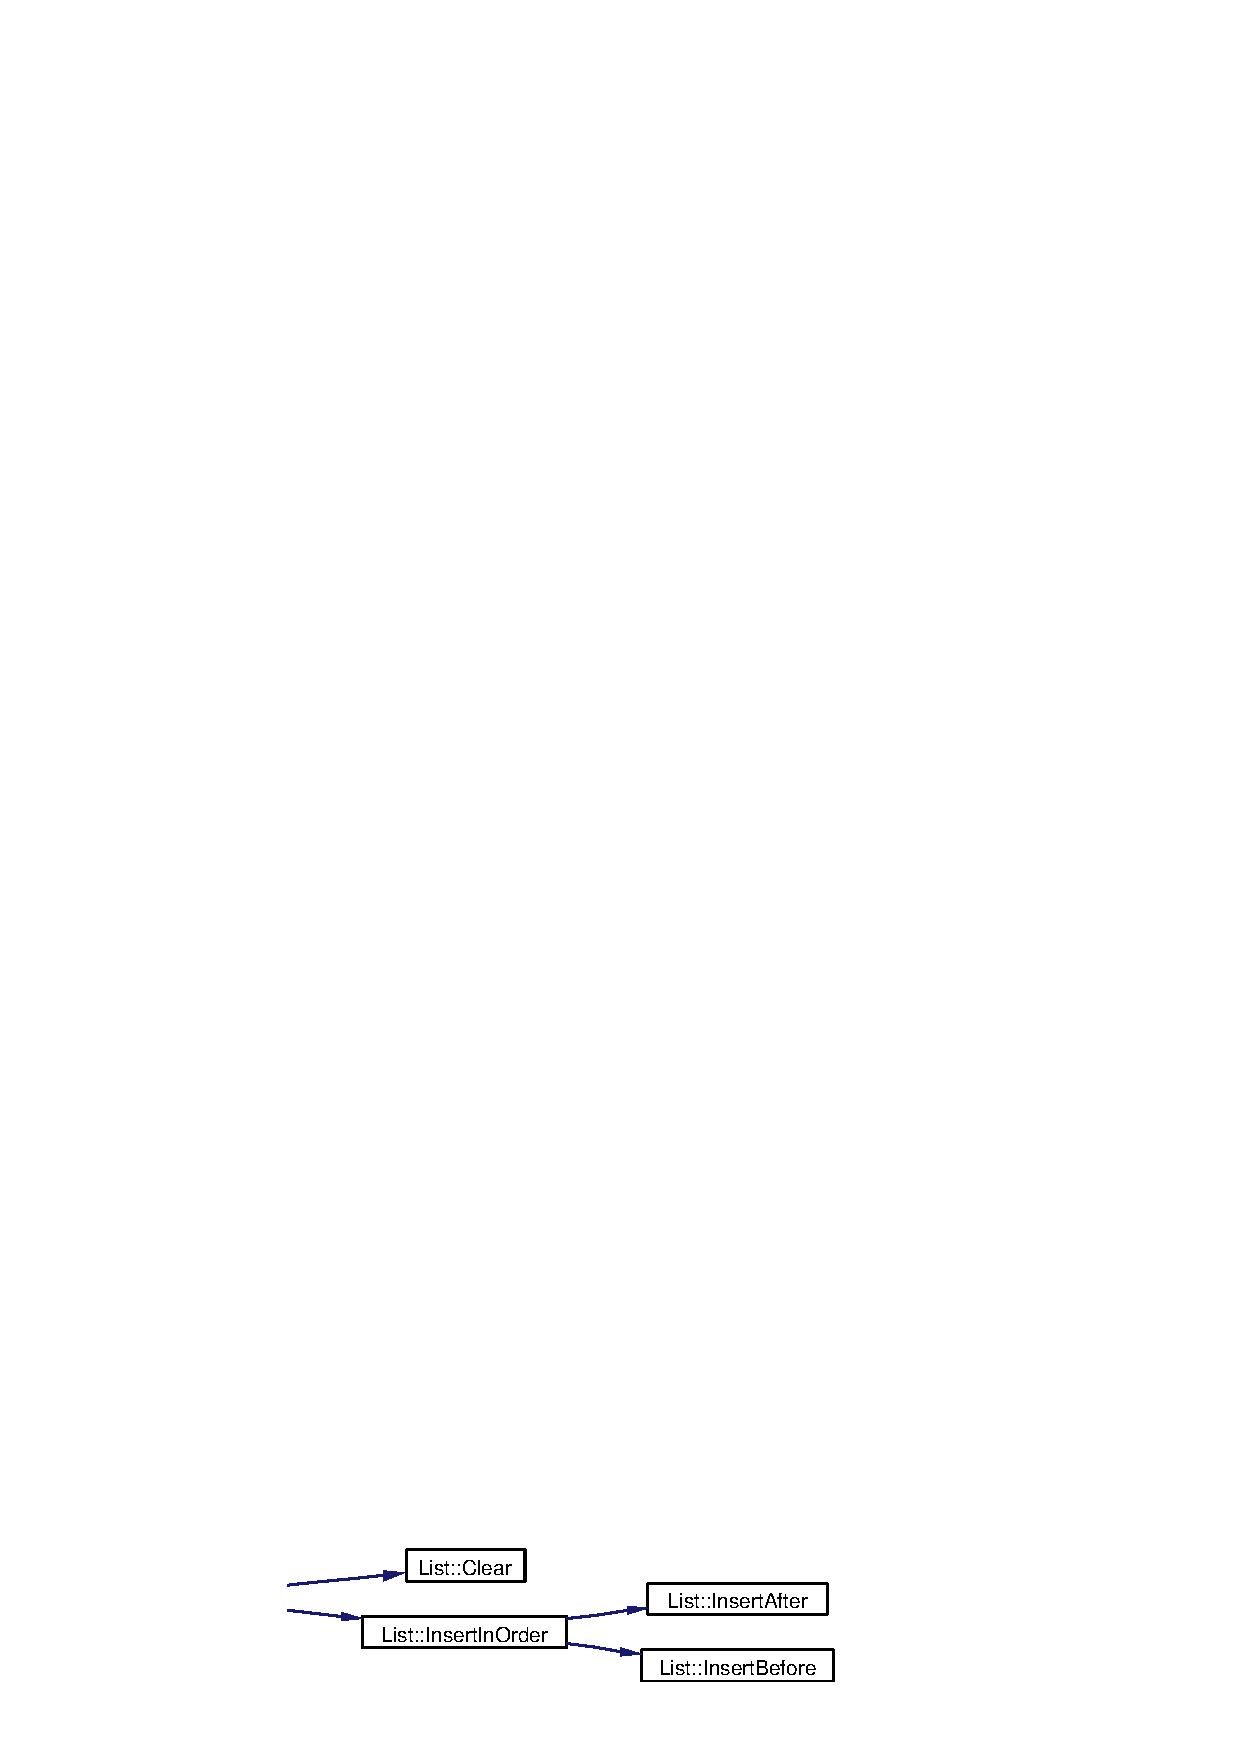
\includegraphics[width=204pt]{classList_a27_cgraph}
\end{center}
\end{figure}
\index{List@{List}!Length@{Length}}
\index{Length@{Length}!List@{List}}
\subsubsection{\setlength{\rightskip}{0pt plus 5cm}template$<$class Etype$>$ int {\bf List}$<$ Etype $>$::Length () const}\label{classList_a17}




Definition at line 568 of file link\-List.h.

References List$<$ Etype $>$::size.

Referenced by Random::Assign\-Prob(), Choose\-L(), Cumul\-Weights(), List$<$ Etype $>$::Pick\-From\-List(), and Event::Stimes().\index{List@{List}!Max@{Max}}
\index{Max@{Max}!List@{List}}
\subsubsection{\setlength{\rightskip}{0pt plus 5cm}template$<$class Etype$>$ Etype {\bf List}$<$ Etype $>$::Max ()}\label{classList_a23}




Definition at line 729 of file link\-List.h.

References List$<$ Etype $>$::current, List$<$ Etype $>$::Node::element, List$<$ Etype $>$::Head(), and List$<$ Etype $>$::size.

Here is the call graph for this function:\begin{figure}[H]
\begin{center}
\leavevmode
\includegraphics[width=100pt]{classList_a23_cgraph}
\end{center}
\end{figure}
\index{List@{List}!Min@{Min}}
\index{Min@{Min}!List@{List}}
\subsubsection{\setlength{\rightskip}{0pt plus 5cm}template$<$class Etype$>$ Etype {\bf List}$<$ Etype $>$::Min ()}\label{classList_a22}




Definition at line 694 of file link\-List.h.

References List$<$ Etype $>$::current, List$<$ Etype $>$::Node::element, List$<$ Etype $>$::Head(), and List$<$ Etype $>$::size.

Referenced by List$<$ Etype $>$::Transpose().

Here is the call graph for this function:\begin{figure}[H]
\begin{center}
\leavevmode
\includegraphics[width=99pt]{classList_a22_cgraph}
\end{center}
\end{figure}
\index{List@{List}!Normalize@{Normalize}}
\index{Normalize@{Normalize}!List@{List}}
\subsubsection{\setlength{\rightskip}{0pt plus 5cm}template$<$class Etype$>$ void {\bf List}$<$ Etype $>$::Normalize ()}\label{classList_a25}




Definition at line 792 of file link\-List.h.

References List$<$ Etype $>$::current, List$<$ Etype $>$::Node::element, List$<$ Etype $>$::Head(), List$<$ Etype $>$::size, and List$<$ Etype $>$::Sum().

Referenced by Cumul\-Weights().

Here is the call graph for this function:\begin{figure}[H]
\begin{center}
\leavevmode
\includegraphics[width=167pt]{classList_a25_cgraph}
\end{center}
\end{figure}
\index{List@{List}!operator++@{operator++}}
\index{operator++@{operator++}!List@{List}}
\subsubsection{\setlength{\rightskip}{0pt plus 5cm}template$<$class Etype$>$ {\bf List}$<$ Etype $>$ \& {\bf List}$<$ Etype $>$::operator++ (int)}\label{classList_a13}




Definition at line 500 of file link\-List.h.

References List$<$ Etype $>$::current, List$<$ Etype $>$::Node::next, and List$<$ Etype $>$::size.\index{List@{List}!operator--@{operator--}}
\index{operator--@{operator--}!List@{List}}
\subsubsection{\setlength{\rightskip}{0pt plus 5cm}template$<$class Etype$>$ {\bf List}$<$ Etype $>$ \& {\bf List}$<$ Etype $>$::operator-- (int)}\label{classList_a14}




Definition at line 515 of file link\-List.h.

References List$<$ Etype $>$::current, List$<$ Etype $>$::head, and List$<$ Etype $>$::Node::next.\index{List@{List}!operator=@{operator=}}
\index{operator=@{operator=}!List@{List}}
\subsubsection{\setlength{\rightskip}{0pt plus 5cm}template$<$class Etype$>$ {\bf List}$<$ Etype $>$ \& {\bf List}$<$ Etype $>$::operator= (const {\bf List}$<$ Etype $>$ \& {\em origlist})}\label{classList_a5}




Definition at line 288 of file link\-List.h.

References List$<$ Etype $>$::Clear(), List$<$ Etype $>$::current, List$<$ Etype $>$::Node::element, List$<$ Etype $>$::head, List$<$ Etype $>$::Node::next, and List$<$ Etype $>$::size.

Here is the call graph for this function:\begin{figure}[H]
\begin{center}
\leavevmode
\includegraphics[width=113pt]{classList_a5_cgraph}
\end{center}
\end{figure}
\index{List@{List}!PickFromList@{PickFromList}}
\index{PickFromList@{PickFromList}!List@{List}}
\subsubsection{\setlength{\rightskip}{0pt plus 5cm}template$<$class Etype$>$ void {\bf List}$<$ Etype $>$::Pick\-From\-List (Etype {\em a\-Low}, Etype {\em a\-High})}\label{classList_a20}




Definition at line 629 of file link\-List.h.

References List$<$ Etype $>$::Head(), List$<$ Etype $>$::Length(), List$<$ Etype $>$::Remove(), List$<$ Etype $>$::Retrieve(), and List$<$ Etype $>$::size.

Here is the call graph for this function:\begin{figure}[H]
\begin{center}
\leavevmode
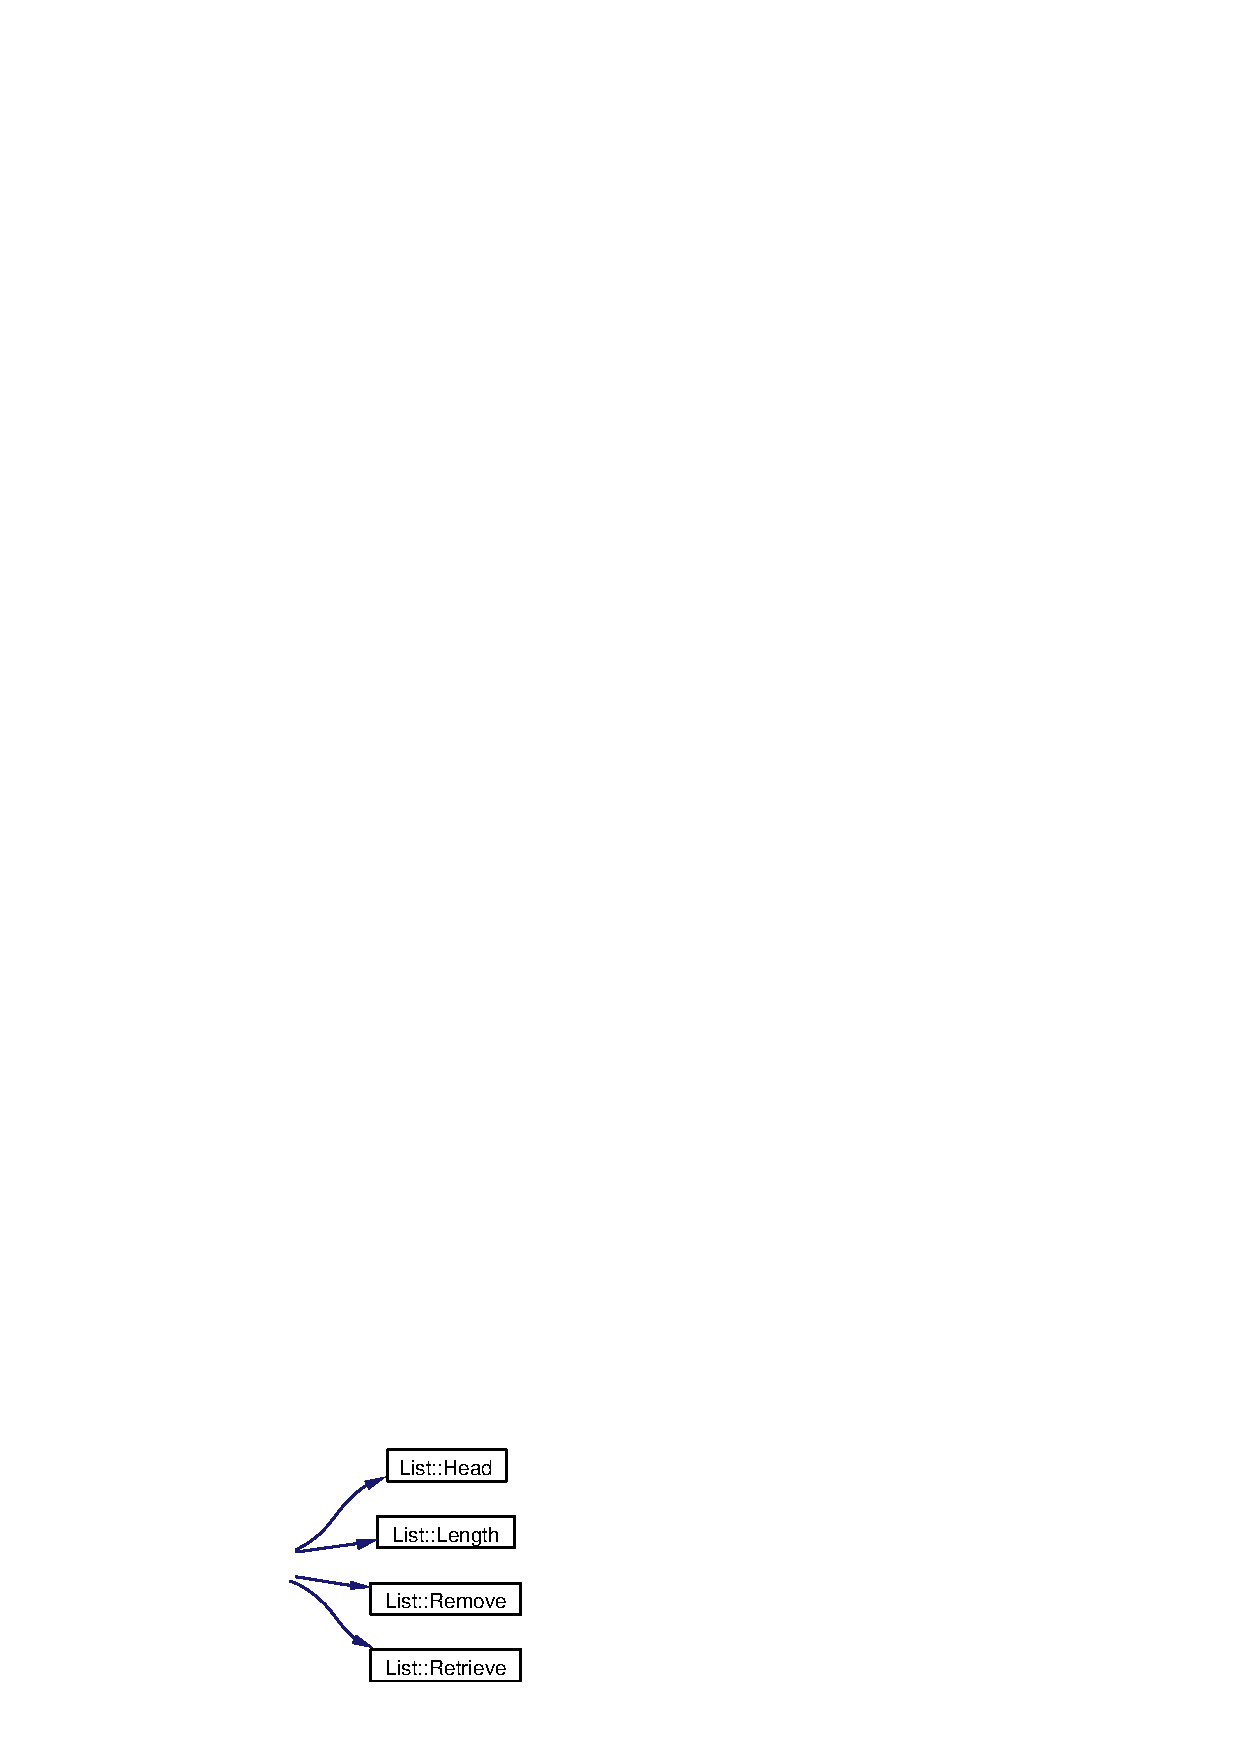
\includegraphics[width=129pt]{classList_a20_cgraph}
\end{center}
\end{figure}
\index{List@{List}!Print@{Print}}
\index{Print@{Print}!List@{List}}
\subsubsection{\setlength{\rightskip}{0pt plus 5cm}template$<$class Etype$>$ void {\bf List}$<$ Etype $>$::Print ()}\label{classList_a18}




Definition at line 580 of file link\-List.h.

References List$<$ Etype $>$::current, List$<$ Etype $>$::Node::element, List$<$ Etype $>$::Head(), and List$<$ Etype $>$::size.

Here is the call graph for this function:\begin{figure}[H]
\begin{center}
\leavevmode
\includegraphics[width=101pt]{classList_a18_cgraph}
\end{center}
\end{figure}
\index{List@{List}!Remove@{Remove}}
\index{Remove@{Remove}!List@{List}}
\subsubsection{\setlength{\rightskip}{0pt plus 5cm}template$<$class Etype$>$ void {\bf List}$<$ Etype $>$::Remove ()}\label{classList_a9}




Definition at line 417 of file link\-List.h.

References List$<$ Etype $>$::current, List$<$ Etype $>$::Node::element, List$<$ Etype $>$::head, List$<$ Etype $>$::Node::next, and List$<$ Etype $>$::size.

Referenced by List$<$ Etype $>$::Pick\-From\-List(), and List$<$ Etype $>$::Sieve().\index{List@{List}!Retrieve@{Retrieve}}
\index{Retrieve@{Retrieve}!List@{List}}
\subsubsection{\setlength{\rightskip}{0pt plus 5cm}template$<$class Etype$>$ Etype {\bf List}$<$ Etype $>$::Retrieve () const}\label{classList_a15}




Definition at line 533 of file link\-List.h.

References List$<$ Etype $>$::current, and List$<$ Etype $>$::Node::element.

Referenced by Choose\-L(), Cumul\-Weights(), GSection(), List$<$ Etype $>$::Pick\-From\-List(), Event::Stimes(), and List$<$ Etype $>$::Sum().\index{List@{List}!Scale@{Scale}}
\index{Scale@{Scale}!List@{List}}
\subsubsection{\setlength{\rightskip}{0pt plus 5cm}template$<$class Etype$>$ void {\bf List}$<$ Etype $>$::Scale ()}\label{classList_a26}




Definition at line 823 of file link\-List.h.

References List$<$ Etype $>$::current, List$<$ Etype $>$::Node::element, List$<$ Etype $>$::Head(), and List$<$ Etype $>$::size.

Here is the call graph for this function:\begin{figure}[H]
\begin{center}
\leavevmode
\includegraphics[width=101pt]{classList_a26_cgraph}
\end{center}
\end{figure}
\index{List@{List}!Sieve@{Sieve}}
\index{Sieve@{Sieve}!List@{List}}
\subsubsection{\setlength{\rightskip}{0pt plus 5cm}template$<$class Etype$>$ void {\bf List}$<$ Etype $>$::{\bf Sieve} ({\bf List}$<$ Etype $>$ \& {\em a\-Sieve})}\label{classList_a19}




Definition at line 604 of file link\-List.h.

References List$<$ Etype $>$::current, List$<$ Etype $>$::Node::element, List$<$ Etype $>$::head, List$<$ Etype $>$::Includes(), List$<$ Etype $>$::Remove(), and List$<$ Etype $>$::size.

Here is the call graph for this function:\begin{figure}[H]
\begin{center}
\leavevmode
\includegraphics[width=108pt]{classList_a19_cgraph}
\end{center}
\end{figure}
\index{List@{List}!Sum@{Sum}}
\index{Sum@{Sum}!List@{List}}
\subsubsection{\setlength{\rightskip}{0pt plus 5cm}template$<$class Etype$>$ Etype {\bf List}$<$ Etype $>$::Sum ()}\label{classList_a21}




Definition at line 659 of file link\-List.h.

References List$<$ Etype $>$::current, List$<$ Etype $>$::Head(), List$<$ Etype $>$::Retrieve(), and List$<$ Etype $>$::size.

Referenced by List$<$ Etype $>$::Normalize().

Here is the call graph for this function:\begin{figure}[H]
\begin{center}
\leavevmode
\includegraphics[width=107pt]{classList_a21_cgraph}
\end{center}
\end{figure}
\index{List@{List}!Tail@{Tail}}
\index{Tail@{Tail}!List@{List}}
\subsubsection{\setlength{\rightskip}{0pt plus 5cm}template$<$class Etype$>$ void {\bf List}$<$ Etype $>$::Tail ()}\label{classList_a12}




Definition at line 486 of file link\-List.h.

References List$<$ Etype $>$::current, List$<$ Etype $>$::Node::next, and List$<$ Etype $>$::size.\index{List@{List}!Transpose@{Transpose}}
\index{Transpose@{Transpose}!List@{List}}
\subsubsection{\setlength{\rightskip}{0pt plus 5cm}template$<$class Etype$>$ void {\bf List}$<$ Etype $>$::Transpose (Etype {\em a\-Start})}\label{classList_a24}




Definition at line 764 of file link\-List.h.

References List$<$ Etype $>$::current, List$<$ Etype $>$::Node::element, List$<$ Etype $>$::Head(), List$<$ Etype $>$::Min(), and List$<$ Etype $>$::size.

Here is the call graph for this function:\begin{figure}[H]
\begin{center}
\leavevmode
\includegraphics[width=157pt]{classList_a24_cgraph}
\end{center}
\end{figure}
\index{List@{List}!Update@{Update}}
\index{Update@{Update}!List@{List}}
\subsubsection{\setlength{\rightskip}{0pt plus 5cm}template$<$class Etype$>$ void {\bf List}$<$ Etype $>$::Update (Etype {\em update\-Elem})}\label{classList_a10}




Definition at line 459 of file link\-List.h.

References List$<$ Etype $>$::current, List$<$ Etype $>$::Node::element, and List$<$ Etype $>$::size.

Referenced by Random::Assign\-Prob(), and Cumul\-Weights().

\subsection{Member Data Documentation}
\index{List@{List}!current@{current}}
\index{current@{current}!List@{List}}
\subsubsection{\setlength{\rightskip}{0pt plus 5cm}template$<$class Etype$>$ {\bf Node} $\ast$ {\bf List}$<$ Etype $>$::{\bf current}\hspace{0.3cm}{\tt  [protected]}}\label{classList_p1}




Definition at line 175 of file link\-List.h.

Referenced by List$<$ Etype $>$::Clear(), List$<$ Etype $>$::Head(), List$<$ Etype $>$::Includes(), List$<$ Etype $>$::Insert\-After(), List$<$ Etype $>$::Insert\-Before(), List$<$ Etype $>$::Insert\-In\-Order(), List$<$ Etype $>$::Insertion\-Sort(), List$<$ Etype $>$::List(), List$<$ Etype $>$::Max(), List$<$ Etype $>$::Min(), List$<$ Etype $>$::Normalize(), List$<$ Etype $>$::operator++(), List$<$ Etype $>$::operator--(), List$<$ Etype $>$::operator=(), List$<$ Etype $>$::Print(), List$<$ Etype $>$::Remove(), List$<$ Etype $>$::Retrieve(), List$<$ Etype $>$::Scale(), List$<$ Etype $>$::Sieve(), List$<$ Etype $>$::Sum(), List$<$ Etype $>$::Tail(), List$<$ Etype $>$::Transpose(), and List$<$ Etype $>$::Update().\index{List@{List}!head@{head}}
\index{head@{head}!List@{List}}
\subsubsection{\setlength{\rightskip}{0pt plus 5cm}template$<$class Etype$>$ {\bf Node}$\ast$ {\bf List}$<$ Etype $>$::{\bf head}\hspace{0.3cm}{\tt  [protected]}}\label{classList_p0}




Definition at line 175 of file link\-List.h.

Referenced by List$<$ Etype $>$::Clear(), List$<$ Etype $>$::Head(), List$<$ Etype $>$::Includes(), List$<$ Etype $>$::Insert\-After(), List$<$ Etype $>$::Insert\-Before(), List$<$ Etype $>$::Insert\-In\-Order(), List$<$ Etype $>$::Insertion\-Sort(), List$<$ Etype $>$::List(), List$<$ Etype $>$::operator--(), List$<$ Etype $>$::operator=(), List$<$ Etype $>$::Remove(), and List$<$ Etype $>$::Sieve().\index{List@{List}!size@{size}}
\index{size@{size}!List@{List}}
\subsubsection{\setlength{\rightskip}{0pt plus 5cm}template$<$class Etype$>$ int {\bf List}$<$ Etype $>$::{\bf size}\hspace{0.3cm}{\tt  [protected]}}\label{classList_p2}




Definition at line 178 of file link\-List.h.

Referenced by List$<$ Etype $>$::Clear(), List$<$ Etype $>$::Insert\-After(), List$<$ Etype $>$::Insert\-Before(), List$<$ Etype $>$::Insert\-In\-Order(), List$<$ Etype $>$::Insertion\-Sort(), List$<$ Etype $>$::Length(), List$<$ Etype $>$::List(), List$<$ Etype $>$::Max(), List$<$ Etype $>$::Min(), List$<$ Etype $>$::Normalize(), List$<$ Etype $>$::operator++(), List$<$ Etype $>$::operator=(), List$<$ Etype $>$::Pick\-From\-List(), List$<$ Etype $>$::Print(), List$<$ Etype $>$::Remove(), List$<$ Etype $>$::Scale(), List$<$ Etype $>$::Sieve(), List$<$ Etype $>$::Sum(), List$<$ Etype $>$::Tail(), List$<$ Etype $>$::Transpose(), and List$<$ Etype $>$::Update().

The documentation for this class was generated from the following file:\begin{CompactItemize}
\item 
{\bf link\-List.h}\end{CompactItemize}
